\documentclass[]{article}
\usepackage{amssymb,amsmath}
\usepackage{hyperref}

\usepackage{todonotes}
\usepackage[margin=2.5cm]{geometry}
\usepackage[super]{natbib}
\bibliographystyle{unsrtnat}

\title{Szilard Intelligence}
\author{Neil D. Lawrence}
\date{9th January 2021}

\begin{document}


\maketitle


\newcommand{\phaseVariables}{\Gamma}
\newcommand{\stateVariables}{X}
\newcommand{\nullVariables}{{X_0}}
\newcommand{\domainVariables}{{X_1}}
\newcommand{\dataVariables}{Y}
\newcommand{\measuredVariables}{S}
\newcommand{\measuredValue}{s}
\newcommand{\parameterVector}{W}
\newcommand{\separability}{{F_S}}
\newcommand{\expDist}[2]{\left\langle #1 \right\rangle_{#2}}
\newcommand{\trueProb}{\mathfrak{P}}
\newcommand{\simProb}{s}
\newcommand{\domainProb}{\mathbb{P}}
\newcommand{\physicsProb}{p}
\newcommand{\approxProb}{q}
\newcommand{\statsProb}{\pi}



\todo{Wonder how this is related to Ashby's concept of "variety",
  e.g. the requisite law of variety:
  \url{https://en.wikipedia.org/wiki/Variety_(cybernetics)}}

\section{Introduction}

The objective of this paper is to provide a mathematical definition of intelligence that grounds our intelligence in the physical sciences. Previous efforts at mathematically defining universal intelligence \citep{Legg-universal07} have reviewed the literature to distil the facets of intelligence, a descriptive approach to a model of intelligence. Our definition is inspired by statistical mechanics descriptions of the universe.  and the simple idea that an intelligent decision is one that achieves a desired state change within the universe with the minimal use of resource. From a physical perspective there are two principal resources we can consider: time and energy. 
\subsection{Energy}

In practice energy is conserved, so the resource of interest is \emph{free energy} the energy available to us to do work.  In statistical physics, we write down the probability of the microstates in a Boltzmann distribution as follows,
\[
\trueProb(\phaseVariables) = \frac{1}{Z_\phaseVariables} \exp(-\beta
E(\phaseVariables)),
\] 
where \(E(\phaseVariables)\) is the \emph{Hamiltonian} which encodes the energy of the system associated with the microstates \(\phaseVariables\) and the partition function is then given by 
\[
Z_\phaseVariables = \sum_\phaseVariables \exp(-\beta E(\phaseVariables)),
\] 
where the \(Z\) comes from the German for ``sum over states'' or
\emph{Zustandssumme}, reflecting Ludwig Boltzmann's Austrian heritage. Boltzmann was the first to make the connection between probability and entropy\citep{Boltzmann-warmetheorie77,}In the
case of continuous systems we have,
\[
Z_{\phaseVariables} = \frac{1}{h^3}\int \exp(-\beta E(\phaseVariables)) \text{d} \phaseVariables
\] 
and \(E(\phaseVariables)\) is the Hamiltonian of the system.

\subsubsection{Total Energy}

Thermodynamics proceeds by considering the total energy of the system, which is defined as the expected energy under the Boltzmann distribution,
\[
U_\phaseVariables = \expDist{E(\phaseVariables)}{\trueProb(\phaseVariables)}.
\] 
The total energy can be decomposed into
\[
U_\phaseVariables = A_\phaseVariables + TS_\phaseVariables,
\] 
where 
\[
A_\phaseVariables = - \frac{1}{\beta}\log Z_\phaseVariables
\] 
is the \emph{Helmholtz free energy} and 
\[ S_\phaseVariables = -k_B
\expDist{\log \trueProb(\phaseVariables)}{\trueProb(\phaseVariables)}
\] 
is the entropy of the system and \(T\) is the temperature. This decomposition is fundamental to thermodynamics, but it is also easily derived mathematically using the definition of the Boltzmann distribution (see \ref{sec-decomposition-of-total-energy}).

This equation expresses a decomposition of the total
energy into the available energy, \(A_\phaseVariables\) and energy
that is not available, \(TS_\phaseVariables\). In terms of the resource we are interested in it is the \emph{free energy}, $A_\phaseVariables$, that we would like to maximise as this is the energy that remains available to us for work.

\subsection{Time}

Beyond available energy, the other other fundamental resource of interest is time. Given two actions that modify the state of the universe with the same resulting change in free energy, we might argue that the action that achieved that state quicker was the more intelligent action. For the moment, however, we will ignore the influence of time, focusing only on the available energy change. 

\subsection{Intelligence and Energy} \label{sec-intelligence-and-energy}

We define an intelligent decision to be one that achieves a desired
change of state in our system with the minimum use of resource. For the
moment, time will not enter our calculations because we will focus on
\emph{thermodynamic equilibria}\footnote{This is equivalent to considering the system in \emph{steady state}}.

Our first step will be to split our phase space into macroscopic variables that we can observe and/or modify and all the other variables, 
$\phaseVariables = \{\stateVariables, \dataVariables\}$, this allows us to write the decomposition of the total energy as
\[
U_{\stateVariables,\dataVariables} =
A_{\stateVariables,\dataVariables} +
TS_{\stateVariables,\dataVariables},
\] 
where 
\[
A_{\stateVariables,\dataVariables} = - \frac{1}{\beta}\log
Z_{\stateVariables,\dataVariables},
\] 
\[
S_{\stateVariables,\dataVariables} = -k_B \expDist{\log
  \trueProb({\stateVariables,\dataVariables})}{\trueProb({\stateVariables,\dataVariables})}
\]
and we have introduced the thermodynamic temperature, $\beta^{-1}=k_B T$.
In thermodynamics we might think of the observable values as
`measurable state variables', whereas the microstates,
$\stateVariables$, are normally considered to be not directly
measurable. In machine learning though, we also might think of
$\stateVariables$ as latent variables and $\dataVariables$ as data, or
potential data. 

In general, we assume that we can interact with our system of interest, so we also assume that some (or all) of these, $\dataVariables$, might be modifyiable. In other words we could fix intervene in our system and set them to particular values (as in e.g. the do-calculus \citep{Pearl-causal95}). Such interventions, or even the act of observation, will have an energy cost. To represent the active interactions with the system we introduce a set of variables,
$\measuredVariables$ is a matrix that indicates if 
a corresponding variable is modified or actively observed. 

We can now denote interactions with the system through changing the
values of $\measuredVariables$. Any such interaction will have an energy cost that we denote $E(\measuredVariables)$.

If we modify or observe our observable states we \emph{instantiate} them observable states. From a
probabilistic perspective, this change is equivalent to
\emph{conditioning} on \(\dataVariables\).

Making an observation or modifying a measurable state in this system is equivalent to conditioning on
\(\dataVariables\). The updated total energy can be written as,
\[
U_{\stateVariables|\dataVariables} =
E(\measuredVariables=\measuredValue) +
\expDist{E({\stateVariables|\dataVariables})}{\trueProb({\stateVariables|\dataVariables})},
\]
where we have used $E(\measuredVariables=\measuredValue)$
to denote the energy associated with making the observation.

We decompose the Hamiltonian into two parts, the first part represents the physics of our measurement, it gives the relationship between the microstates and our observable variables,
\(E(\dataVariables|\stateVariables)\) and the second is the Hamiltonian of the microstates, \(E(\stateVariables)\), this allows us to write
\[
\mathbb{P}({\stateVariables|\dataVariables}) =
\frac{1}{Z_{\stateVariables|\dataVariables}} \exp\left(-\beta
E(\dataVariables|\stateVariables) -\beta E(\stateVariables)\right)
\] 
where the partition function is given by
\[
Z_{\stateVariables|\dataVariables} = \int \exp\left(-\beta
E(\dataVariables|\stateVariables) -\beta E(\stateVariables)\right)
\text{d}\stateVariables.
\] 

So after intervening in our system, and taking a set of measurements or modifying the observable variables, the new total energy of the system is,
\[
U_{\stateVariables|\dataVariables} =
E(\measuredVariables=\measuredValue) +
A_{\stateVariables|\dataVariables} +
TS_{\stateVariables|\dataVariables}
\] 
where 
\[
A_{\stateVariables|\dataVariables} = - \frac{1}{\beta}\log
Z_{\stateVariables|\dataVariables}
\] 
and 
\[
S_{\stateVariables|\dataVariables} = -k_B \expDist{\log
  \trueProb({\stateVariables|\dataVariables})}{\trueProb({\stateVariables|\dataVariables})}.
\]

This is the representation of our universe in its updated state. We can now compute how the available energy has changed by subtracting the available energy in our original universe from the available energy in our updated universe, subtracting, $\Delta A_{Y} = A_{\stateVariables|\dataVariables} -
  A_{\stateVariables,\dataVariables}$, using standard rules of probability this gives
\begin{align*}
 \Delta A_{Y}  = & -\frac{1}{\beta} \log
  \frac{Z_{\stateVariables|\dataVariables}}{Z_{\stateVariables,\dataVariables}}\\ &
  -\frac{1}{\beta} \log \trueProb(\dataVariables)
\end{align*}
which is also recognised as the Shannon information we gain through the observation \citep{Shannon-info48} under Boltzmann's distribution. The thermodynamic temperature, $\beta$, relates the dimensionless information to the available energy gain in Joules. Note that this connection between thermodynamics and information predates Shannon. It goes back to the work of Szilard\citep{Szilard-intelligenter29} who was considering a thought experiment known as \emph{Maxwell's demon}\citep{Maxwell-theory71,Leff-maxwell90}. In the thought experiment a demon transgresses the second law of thermodynamics by partitioning an isolated box of gas into two parts. The demon allows high energy particles to pass from the left hand side to the right hand side through opening a slot when they approach the partition. Similarly low energy particles are allowed to pass from right to left. In this way the entropy of the gas in the box appears to be reduced. 

Maxwell included the demon in his book which gave his theory of heat\citep{Maxwell-theory71}. He was illustrating that the second law holds only in expectation, but the thought experiment intrigued the community and was developed further by Szilard\citep{Szilard-intelligenter29}. Szilard reduced the system to one containing a single particle (now known as a Szilard engine). He showed that the demon introduces information to the system which counteracts the reduction in entropy. In this way Szilard introduced an equivalence between thermodynamic entropy and information (through the thermodynamic temperature, $\beta$).

The second law of thermodynamics states that entropy cannot decrease as time proceeds in a forward direction. It is through the second law that we understand the impossibility of perpetual motion machines and the irreversibility of certain physical processes. So it is from Maxwell's demon and Szilard's engine that we draw our inspiration for our  definition of intelligence. For this reason we call it Szilard intelligence.

In physics, much of the discussion of Szilard's paper dwells on where energy is required for the demon to store or acquire the information. We might think of this as an attempt to lower bound $E(\measuredVariables=\measuredValue)$. In this paper, our focus is different. We assume that any interaction with the system will \emph{may} require energy (whether through measurements or interventions). So the available energy gain needs to be traded off against the cost of intervention given by $E(\measuredVariables=\measuredValue)$. 

This is the fundamental relation between information and energy that
we need to pursue our definition of intelligence. By measuring our
system we gain available energy. If the cost of the measurement is
less than the amount of available energy we gain, then this is an
action worth taking.

\subsection{Intelligence Quotient}

We define a dimensionless quotient to represent the Szilard intelligence of an action
(where action is taken to mean a change of $\measuredVariables$) to be,
\[
I = \frac{\exp(-\beta E(\measuredVariables=\measuredValue))}{\trueProb(\dataVariables)},
\]
where $\beta$ is again the thermodynamic temperature \(\beta = \frac{1}{Tk_B}\). A demon that was infringing the second law of thermodynamics would have a Szilard coefficient greater than one. What Szilard's work suggested is that for the second law to be preserved, the Szilard coefficient must be upper bounded by 1. We can express the available energy gain in terms of the logarithm of the quotient as follows,
\[
\Delta A_\dataVariables = T k_B\log I,
\]
which since $I\leq 1$ is always zero or negative in sign. 

The upper bound on the Szilard coefficient provides a thermodynamic upper limit on the intelligence of a decision given by the second law. 

Note that our definition of the Szilard coefficient for scoring intelligence doesn't require us to define a mechanism by which the intelligent action is occurring, it merely relates the measurable and manipulable states $\dataVariables$, to the energy of the system.

The most intelligent action is the one that achieves the desired state $\dataVariable = \dataValue$ with the largest Szilard coefficient which corresponds to the smallest loss in available energy. The optimal action under the Szilard coefficient involves trading of the information associated with a particular state, $-\log \trueProb(\dataVariables)$, with the energy cost of achieving that state.

In practice, we typically won't have access to the distribution, $\trueProb(\cdot)$, so we cannot optimise our actions directly with respect to the Szilard coefficient. In the next section, we introduce a lower bound on the Szilard coefficient, one that is derived through introducing a physical simulation, $\simProb(\stateVariables)$.

\subsection{Lower Bound}

The upper bound on the Szilard coefficient is given by the second law. To obtain a lower bound on the coefficient, we must first \emph{upper} bound $\log \trueProb(\dataVariables)$. In Appendix \ref{sec-}
\[
\log \trueProb(\dataVariables) \leq \log \physicsProb(\dataVariables)
+
\text{KL}(\simProb(\stateVariables)||\trueProb(\stateVariables|\dataVariables)).
\]
where we have introduced a the distribution $\simProb(\stateVariables)$ to represent our \emph{simulation} of  $\stateVariables$. For our purposes, a simulation is our best approximation of the physical world according to our understanding. The model, $\physicsProb(\dataVariables)$ is defined as,
$$
\physicsProb(\dataVariables) = \frac{\exp(-\beta \expDist{E(\dataVariables|\stateVariables)}{\simProb(\stateVariables)}}{Z^\prime_\dataVariables}
$$
where $Z^\prime_\dataVariables = \sum_\dataVariables \exp(-\beta \expDist{E(\dataVariables|\stateVariables)}{\simProb(\stateVariables)}$. 

The notation $\text{KL}(\simProb(\cdot)||\trueProb(\cdot))$ represents the Kullback Leibler (KL) divergence\citep{Kullback-info51} between the two distributions, $\simProb(\cdot)$ and $\trueProb(\cdot)$ and is defined by,
$$
\text{KL}(\simProb(\stateVariables) || \trueProb(\stateVariables)) = \sum_\stateVariables \simProb(\stateVariables) \log\frac{\simProb(\stateVariables)}{\trueProb(\stateVariables)} \geq 0.
$$
The KL divergence is a standard information theoretic measure of divergence between two distributions. In our derivations we will commonly make use of \emph{fidelity}. We define the $\exp\left(-
\text{KL}(\simProb(\stateVariables)||\trueProb(\stateVariables|\dataVariables))\right)$
to be the \emph{contextual} simulation fidelity, $F_C$,
\[
\log F_C =
-\text{KL}(\simProb(\stateVariables)||\trueProb(\stateVariables|\dataVariables)).
\]
and we can now lower bound the Szilard coefficient,
\[
I \geq F_C \frac{\exp\left(-E(\measuredVariables=\measuredValue)\right)}{\physicsProb(\dataVariables)}.
\]


\subsection{Maximizing the Bound on the Szilard Coefficient}

The bound can be tightened by maximising with respect to $\simProb(\stateVariables)$, which in turn gives us the optimal form of $\physicsProb(\dataVariables)$. The lower bound on the log intelligence quotient is given by,
\[
\log I \geq - \log \physicsProb(\dataVariables) -\text{KL}(\simProb(\stateVariables)||\trueProb(\stateVariables|\dataVariables)) - \beta E(\measuredVariables_\dataVariables = \textbf{1})
\]
recalling that $\log \physicsProb(\dataVariables) = \frac{\exp\left(-\beta\expDist{E(\dataVariables|\stateVariables)}{\simProb(\stateVariables)}\right)}{Z^\prime_\dataVariables}$ and focusing on the terms that are dependent on $\simProb(\stateVariables)$ we have,
\[
\log I \geq \beta \expDist{E(\stateVariables)}{\simProb(\stateVariables)} - \expDist{\log \simProb(\stateVariables)}{\simProb(\stateVariables)} + \text{const.},
\]
where $\text{const.} = \log Z^\prime_Y - \log Z_{\stateVariables|\measuredVariables}$. This can be maximized by setting,
\[
\simProb(\stateVariables) = \trueProb(\stateVariables)
\]
giving us the unsurprising conclusion that the lower bound on the Szilard coefficient quotient is maximised by setting our simulation to be equal to the true distribution of the microstates, $\trueProb(\stateVariables)$, at which point we recover the true Szilard coefficient.

However, since our system is unbounded in scope, and $\stateVariables$ involves all microstates of the Universe, this is quite impractical. So our first step will be to constrain our simulation such that it focuses on variables of interest.

\subsection{Null Space and Domain Space}

So far we have considered a model that contains all the microstates of the Universe, $\stateVariables$. But in practice, when modelling we normally focus on a particular domain. For example, in climate modelling we develop detailed models of the oceans independently from models of the chemistry of the upper atmosphere. Where these two models interact, they do so at defined interfaces. To reflect this we divide the state space into two parts, we call one the null space, and denote it by $\nullVariables$. These are the microstates in the Universe that we'd prefer to ignore in the simulation we're focused on. The second part we call the domain space, which we denote by $\domainVariables$. These are the microstates that we consider directly relevant for the problem at hand. 

As in the case of the climate model separation, we expect to have have different simulations for different contexts. So that we can factorise our universe into different simulations for use in different contexts, we then make the assumption that
\[
\simProb(\stateVariables) = \simProb(\nullVariables) \simProb(\domainVariables)
\]
and we impose this as a constraint when maximising the lower bound on the intelligence quotient.

Under this constraint, we obtain the following form for $\simProb(\domainVariables)$ (see Appendix \ref{sec-optimal-form-of-independent-simulation}),
\[
\simProb(\domainVariables) = \frac{\exp \left(-\beta E^\prime(\domainVariables)\right)}{Z^\prime_\domainVariables},
\]
where we have introduced $E^\prime(\domainVariables) = \expDist{E(\stateVariables)}{\simProb(\nullVariables)}$ as well as the domain simulation's partition function, $Z^\prime_\domainVariables$.

Note that despite our independence assumption between the null space and the domain simulation there is an interdependence between the optimal form for $\simProb(\domainVariables)$ and $\simProb(\nullVariables)$. 

Using our factorised form we can write the lower bound on the Szilard coefficient as (see Appendix \ref{sec-optimal-form-of-independent-simulation}),
$$
\log I \geq -\log \physicsProb(\dataVariables) + \log F_\domainVariables  + \log \separability  -\beta E(\measuredVariables_\dataVariables=\textbf{1})
$$
where we have introduced the \emph{separability}, $\separability$,
$$
\log \separability = - \text{KL}\left(\simProb(\domainVariables)\simProb(\nullVariables)||\trueProb(\domainVariables,\nullVariables)\right)
$$
which represents how separable our choice of domain space and null space are in reality. If $\separability=1$ then the null space and domain space are fully separable. This would occur, for example, if the domain variables were isolated from the null space. We have also defined the \emph{domain fidelity},
$$
\log F_\domainVariables = - \expDist{\text{KL}\left(\simProb(\domainVariables) || \frac{\trueProb(\dataVariables | \domainVariables,\nullVariables)\simProb(\domainVariables)}{\trueProb(\dataVariables)}\right)}{\simProb(\nullVariables)},
$$
which represents the fidelity of our domain simulation to the as the domain fidelity. We now define,
$$
\domainProb(\dataVariables | \domainVariables) = \frac{\exp\expDist{\log \trueProb(\dataVariables | \domainVariables,\nullVariables)}{\simProb(\nullVariables)}}{Z^\prime_{\dataVariables|\domainVariables}}
$$
and 
$$
\domainProb(\domainVariables | \dataVariables) = \frac{\trueProb(\dataVariables | \domainVariables)\simProb(\domainVariables)}{\trueProb(\dataVariables)}
$$
giving
$$
\log F_\domainVariables = - \text{KL}\left(\simProb(\domainVariables) || \domainProb(\domainVariables | \dataVariables)\right)}  - \log \frac{Z^\prime_{\dataVariables|\domainVariables}}{ Z_{\dataVariables|\stateVariables}}  ,
$$
If the domain variables are selected such that,
$$
\trueProb(\dataVariables | \domainVariables, \nullVariables) = \trueProb(\dataVariables |\domainVariables)
$$
then we can write
$$
\log F_\domainVariables = - \text{KL}\left(\simProb(\domainVariables) || \domainProb(\domainVariables | \dataVariables) \right).
$$

\section{Parameters}

We now introduce a set of auxiliary variables, $\parameterVector$. These auxiliary variables augment the domain distribution,
\[
\domainProb(\domainVariables | \dataVariables) = \int \domainProb(\domainVariables, \parameterVector | \dataVariables) \text{d} \parameterVector,
\]
allowing us to lower bound the logarithm of the domain probability,
\[
\log \domainProb(\domainVariables | \dataVariables) \geq \int \simProb(\parameterVector|\domainVariables) \log \frac{\domainProb(\domainVariables, \parameterVector | \dataVariables)}{\simProb(\parameterVector|\domainVariables)} \text{d}\parameterVector,
\]
which in turn allows us to lower bound the domain fidelity, 
\[
\log F_\domainVariables = \int \simProb(\domainVariables) \log \frac{\domainProb(\domainVariables | \dataVariables)}{\simProb(\domainVariables)} \geq \int \simProb(\parameterVector,\domainVariables) \log \frac{\domainProb(\domainVariables, \parameterVector | \dataVariables)}{\simProb(\parameterVector,\domainVariables)} \text{d}\parameterVector.
\]
If we assume that we have introduced $\parameterVector$ such that $\domainProb(\domainVariables, \parameterVector| \dataVariables)$ can be decomposed as follows,
\[
\domainProb(\domainVariables, \parameterVector| \dataVariables) = \domainProb(\domainVariables| \parameterVector, \dataVariables) \trueProb(\parameterVector)
\]
then we can rewrite as
\[
\log F_\domainVariables \geq \int \simProb(\parameterVector) \log \frac{\trueProb(\parameterVector)}{\simProb(\parameterVector)}\text{d} \parameterVector + \int \simProb(\parameterVector) \int \simProb(\domainVariables|\parameterVector) \log \frac{\domainProb(\domainVariables|\parameterVector, \dataVariables)}{\simProb(\domainVariables|\parameterVector)} \text{d} \domainVariables \text{d}\parameterVector,
\]
or in terms of KL divergences,
\begin{align*}
\log F_\domainVariables \geq & -\text{KL}\left(\simProb(\parameterVector)|| \trueProb(\parameterVector)\right) - \expDist{ \text{KL}\left(\simProb(\domainVariables|\parameterVector) || \domainProb(\domainVariables|\parameterVector, \dataVariables) \right)}{ \simProb(\parameterVector)} \\
\log F_\domainVariables \geq & \log F_\parameterVector + \log R_{\domainVariables|\parameterVector}
\end{align*}
which in turn implies that
$$
F_\domainVariables \geq F_\parameterVector R_{\domainVariables|\parameterVector}
$$
where $F_\parameterVector$ is the parameter fidelity and $R_{\domainVariables|\parameterVector}$ is the representability. 

Parameterizing the model has allowed us to decompose the domain fidelity into a parameter fidelity and a representability. To see why we call $F_{\domainVariables |\parameterVector}$ the representability, we first minimizing the lower bound on the intelligence quotient with respect to $\simProb(\domainVariables | \parameterVector)$ and we recover,
$$
\simProb(\domainVariables | \parameterVector) = \domainProb(\domainVariables | \parameterVector).
$$
In which case the representability is given by, 
$$
\log R_{\domainVariables | \parameterVector} = \expDist{ \text{KL}\left(\domainProb(\domainVariables|\parameterVector) || \domainProb(\domainVariables|\parameterVector, \dataVariables) \right)}{ \simProb(\parameterVector)}.
$$
This KL divergence will be zero (and the representability 1) only if conditioning on $\dataVector$ does not change the domainprobability. In other words if $\parameterVector$ renders the domain variables conditionally independent of the data. In other words, storing the parameters is sufficient for us to have all the information about the domain variables, we don't need to store the data itself. For this to happen $\parameterVector$ would have to be sufficiently large to represent all the information in $\dataVector$.
\todo{I think this is all true. Firstly, the minima of the bound (but it relies on $E(Y|X)$ in $p(Y)$ matching that in $\domainProb()$. And secondly that this implies conditional independence if W is large enough ... might need some conditions on a DAG between W, X1 and Y.} 

Minimizing the lower bound on the intelligence quotient with respect to $\simProb(\parameterVector)$ recovers ...
\todo{Need to check what happens here ...} 

\section{Model Selection}

In practice, we want to find the tightest bound on the intelligence ratio. Above we've shown what the form 


Some thoughts:

\begin{enumerate}
    \item Choose parameters such that $\physicsProb(\dataVariables|\parameterVector) = \prod_{i=1}^n \physicsProb(\dataPoint_i |\parameterVector)$
    \item Choosing robust models ... what about heavy tailed vs light tailed $\physicsProb(\dataPoint_i |\parameterVector)$. 
\end{enumerate}

Also for a fixed data set $\dataVariables$, the actual intelligence quotient is fixed. And we are supposed to be computing a lower bound. 

Imagine we have two models, and one model has a higher negative log probability than the other. It doesn't mean it's got a higher intelligence quotient, because that's fixed. Instead, it means our estimate of the intelligence coefficient is likely to be over optimistic. 

It feels likely there's some minimax stuff going on here. We want the model $\physicsProb(\dataVariables)$ which minimise the maximum ... because this will be the one with the highest fidelity and representability. Need to formalise that argument.

\section{Likelihood Ratio Tests}

\todo{Check what happens for likelihood ratio test.}

\subsection{Speculative on Naming}

Spilt the statistical model mismatch into two terms that represent how
'correct' and how 'consistent' the statistical model is.

Correctness represents the ability of the model to reconstruct the
information about domain variables, \(\domainVariables\), that is
provided by the data, \(\dataVariables\), through the parameters,
\(\parameterVector\), alone. The value of
\(B^\prime_{\domainVariables|\dataVariables}\) increases with
incorrectness.

Consistency reflects how likely different data sets are to give us
different parameters. is the relative entropy (KL divergence) between
the parameters of the statistical model,
\(\statsProb(\parameterVector|\dataVariables)\), and the physical model,
\(\physicsProb(\parameterVector|\dataVariables)\).

\bibliography{information-engine.bib}

\appendix

\section{Decomposition of Total Energy} \label{sec-decomposition-of-total-energy}

The total energy of a system ...

\section{Lower Bound on $-\log \trueProb(\dataVariable)$} \label{sec-upper-bound-log-prob}

Rewrite $\log \trueProb(\dataVariables)$ as
\begin{align}
    \log \trueProb(\dataVariables) & =
    \expDist{\trueProb(\dataVariables,
      \stateVariables)}{\simProb(\stateVariables )} + \expDist{\log
      \simProb(\stateVariables)}{\simProb(\stateVariables)} +
    \text{KL}(\simProb(\stateVariables)||\trueProb(\stateVariables|\dataVariables))
    \nonumber \\ & = -\beta\expDist{ E(\dataVariables |
      \stateVariables)}{\simProb(\stateVariables)}
    -\beta\expDist{E(\stateVariables)}{\simProb(\stateVariables)} -
    \log Z_{\stateVariables,\dataVariables} + \expDist{\log
      \simProb(\stateVariables)}{\simProb(\stateVariables)} +
    \text{KL}(\simProb(\stateVariables)||\trueProb(\stateVariables|\dataVariables)) \label{eqn-true-log-likelihood-1}
\end{align}
and then rewrite the log partition function of the system as follows,
\[
- \log Z_{\stateVariables,\dataVariables} =
\beta\expDist{E(\dataVariables |
  \stateVariables)}{\simProb(\stateVariables)\physicsProb(\dataVariables)}
+ \beta\expDist{E(\stateVariables)}{\simProb(\stateVariables )} +
\expDist{\log \trueProb(\dataVariables)}{\physicsProb(\dataVariables)}
-\expDist{\log \simProb(\stateVariables)}{\simProb(\stateVariables)} -
\expDist{\text{KL}(\simProb(\stateVariables) ||
  \physicsProb(\stateVariables |
  \dataVariables))}{\physicsProb(\dataVariables)}
\]
which substituting into (\ref{eqn-true-log-likelihood-1}) gives
\[
\log \trueProb(\dataVariables) = \log \physicsProb(\dataVariables) +
\text{KL}(\simProb(\stateVariables)||\trueProb(\stateVariables|\dataVariables))
- \text{KL}(\physicsProb(\dataVariables) || \trueProb(\dataVariables))
- \expDist{\text{KL}(\simProb(\stateVariables) ||
  \trueProb(\stateVariables |
  \dataVariables))}{\physicsProb(\dataVariables)}
\]

\subsection{Global and Local Simulations}

The two different simulation fidelities represent a fundamental
tension in modelling. The global simulation fidelity gives us a
simulation that tries to be valid across the different data that we
might observe, $\trueProb(\dataVariables)$. The local simulation
fidelity is specific to the data we have, $\dataVariables$. The global
simulation fidelity is associated with our global understanding of
physical laws. The contextual simulation fidelity is associated with
the particular circumstance we currently find ourselves in,
\[
\log F_C =
-\text{KL}(\simProb(\stateVariables)||\trueProb(\stateVariables|\dataVariables)).
\]

The global simulation fidelity considers
\begin{figure}
    \centering
    \def\svgwidth{\textwidth}
   %% Creator: Inkscape 1.0.2 (e86c8708, 2021-01-15), www.inkscape.org
%% PDF/EPS/PS + LaTeX output extension by Johan Engelen, 2010
%% Accompanies image file 'py-bounds.pdf' (pdf, eps, ps)
%%
%% To include the image in your LaTeX document, write
%%   \input{<filename>.pdf_tex}
%%  instead of
%%   \includegraphics{<filename>.pdf}
%% To scale the image, write
%%   \def\svgwidth{<desired width>}
%%   \input{<filename>.pdf_tex}
%%  instead of
%%   \includegraphics[width=<desired width>]{<filename>.pdf}
%%
%% Images with a different path to the parent latex file can
%% be accessed with the `import' package (which may need to be
%% installed) using
%%   \usepackage{import}
%% in the preamble, and then including the image with
%%   \import{<path to file>}{<filename>.pdf_tex}
%% Alternatively, one can specify
%%   \graphicspath{{<path to file>/}}
%% 
%% For more information, please see info/svg-inkscape on CTAN:
%%   http://tug.ctan.org/tex-archive/info/svg-inkscape
%%
\begingroup%
  \makeatletter%
  \providecommand\color[2][]{%
    \errmessage{(Inkscape) Color is used for the text in Inkscape, but the package 'color.sty' is not loaded}%
    \renewcommand\color[2][]{}%
  }%
  \providecommand\transparent[1]{%
    \errmessage{(Inkscape) Transparency is used (non-zero) for the text in Inkscape, but the package 'transparent.sty' is not loaded}%
    \renewcommand\transparent[1]{}%
  }%
  \providecommand\rotatebox[2]{#2}%
  \newcommand*\fsize{\dimexpr\f@size pt\relax}%
  \newcommand*\lineheight[1]{\fontsize{\fsize}{#1\fsize}\selectfont}%
  \ifx\svgwidth\undefined%
    \setlength{\unitlength}{841.88976378bp}%
    \ifx\svgscale\undefined%
      \relax%
    \else%
      \setlength{\unitlength}{\unitlength * \real{\svgscale}}%
    \fi%
  \else%
    \setlength{\unitlength}{\svgwidth}%
  \fi%
  \global\let\svgwidth\undefined%
  \global\let\svgscale\undefined%
  \makeatother%
  \begin{picture}(1,0.70707071)%
    \lineheight{1}%
    \setlength\tabcolsep{0pt}%
    \put(0,0){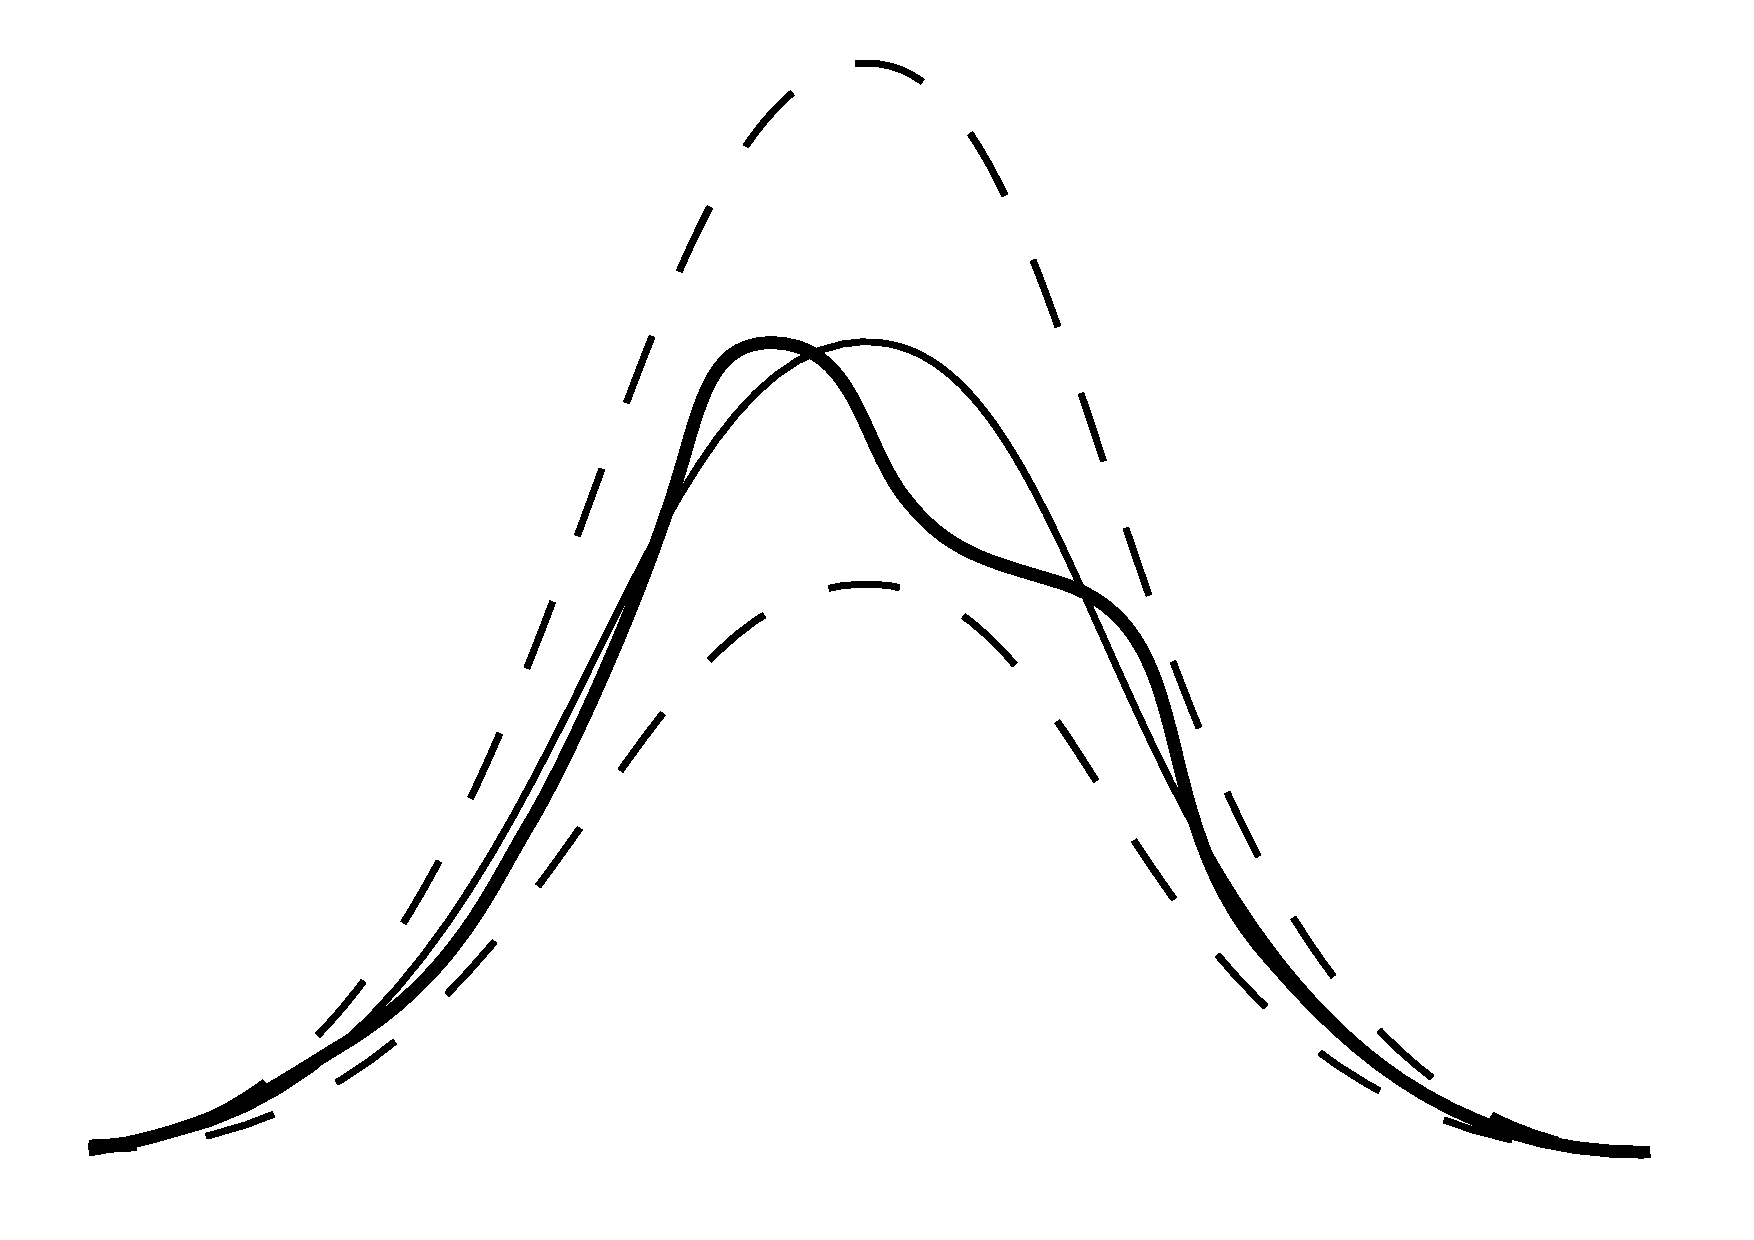
\includegraphics[width=\unitlength,page=1]{py-bounds.pdf}}%
    \put(0.39432495,0.40447998){$\trueProb(Y)$}%
    \put(0.40333575,0.27675171){$F_C \physicsProb(Y)$}%
    \put(0.67081228,0.6197671){$\frac{1}{F_G}\physicsProb(Y)$}%
    \put(0.48646448,0.53538479){$p(Y)$}%
  \end{picture}%
\endgroup%

    \caption{Visualisation of the lower and upper bound on
      $\trueProb(\dataVariables)$ to highlight how the approximation,
      $\physicsProb(\dataVariables)$, corresponds to the bounds
      combining with the fidelities, $F_C$.}
    \label{fig-py-bounds}
\end{figure}



\begin{figure}
  \centering
  \def\svgwidth{\textwidth}
    %% Creator: Inkscape 1.0.2 (e86c8708, 2021-01-15), www.inkscape.org
%% PDF/EPS/PS + LaTeX output extension by Johan Engelen, 2010
%% Accompanies image file 'log-py-bounds.pdf' (pdf, eps, ps)
%%
%% To include the image in your LaTeX document, write
%%   \input{<filename>.pdf_tex}
%%  instead of
%%   \includegraphics{<filename>.pdf}
%% To scale the image, write
%%   \def\svgwidth{<desired width>}
%%   \input{<filename>.pdf_tex}
%%  instead of
%%   \includegraphics[width=<desired width>]{<filename>.pdf}
%%
%% Images with a different path to the parent latex file can
%% be accessed with the `import' package (which may need to be
%% installed) using
%%   \usepackage{import}
%% in the preamble, and then including the image with
%%   \import{<path to file>}{<filename>.pdf_tex}
%% Alternatively, one can specify
%%   \graphicspath{{<path to file>/}}
%% 
%% For more information, please see info/svg-inkscape on CTAN:
%%   http://tug.ctan.org/tex-archive/info/svg-inkscape
%%
\begingroup%
  \makeatletter%
  \providecommand\color[2][]{%
    \errmessage{(Inkscape) Color is used for the text in Inkscape, but the package 'color.sty' is not loaded}%
    \renewcommand\color[2][]{}%
  }%
  \providecommand\transparent[1]{%
    \errmessage{(Inkscape) Transparency is used (non-zero) for the text in Inkscape, but the package 'transparent.sty' is not loaded}%
    \renewcommand\transparent[1]{}%
  }%
  \providecommand\rotatebox[2]{#2}%
  \newcommand*\fsize{\dimexpr\f@size pt\relax}%
  \newcommand*\lineheight[1]{\fontsize{\fsize}{#1\fsize}\selectfont}%
  \ifx\svgwidth\undefined%
    \setlength{\unitlength}{841.88976378bp}%
    \ifx\svgscale\undefined%
      \relax%
    \else%
      \setlength{\unitlength}{\unitlength * \real{\svgscale}}%
    \fi%
  \else%
    \setlength{\unitlength}{\svgwidth}%
  \fi%
  \global\let\svgwidth\undefined%
  \global\let\svgscale\undefined%
  \makeatother%
  \begin{picture}(1,0.70707071)%
    \lineheight{1}%
    \setlength\tabcolsep{0pt}%
    \put(0,0){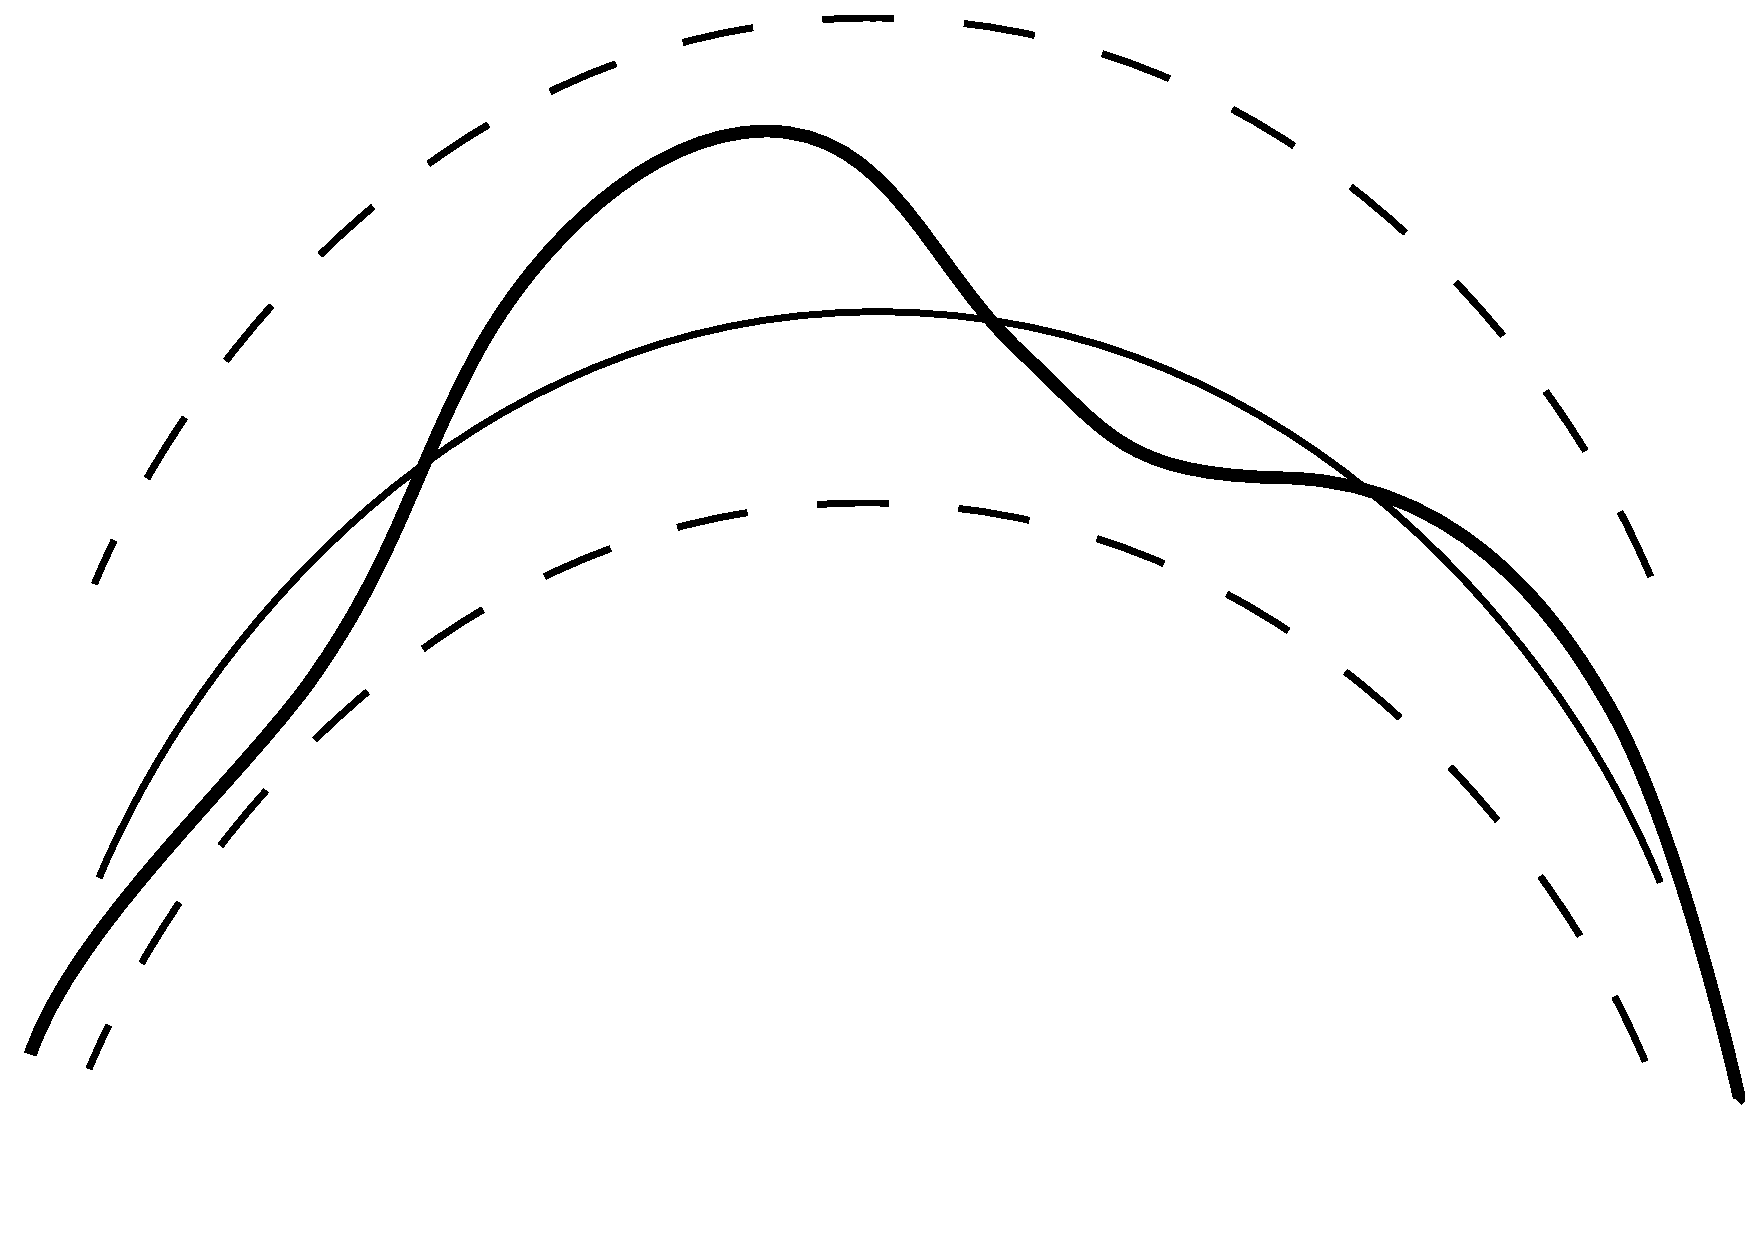
\includegraphics[width=\unitlength,page=1]{./diagrams/log-py-bounds.pdf}}%
    \put(0.55054713,0.58056959){\Large $\log \trueProb(\dataVariables)$}%
    \put(0.31892536,0.34449357){\Large $\log \physicsProb(\dataVariables) + \log F_C$}%
    \put(0.67081228,0.66609147){\Large $\log \physicsProb(\dataVariables) - \log F_G$}%
    \put(0.39197527,0.46832211){\Large $\log \physicsProb(\dataVariables)$}%
  \end{picture}%
\endgroup%

    \caption{Visualisation of the lower and upper bound on $\log
      \trueProb(\dataVariables)$ to highlight how the approximation,
      $\log \physicsProb(\dataVariables)$, corresponds to the bounds
      combining with the fidelities, $\log F_C$ and $\log F_G$.}
    \label{fig-log-py-bounds}
\end{figure}
=======
\section{Optimal form of Independent Simulation} \label{sec-optimal-form-of-independent-simulation}


$$
\log I \geq -\log \physicsProb(\dataVariables) - \expDist{\text{KL}\left(\simProb(\domainVariables) || \frac{\trueProb(\dataVariables | \domainVariables,\nullVariables)\simProb(\domainVariables)}{\trueProb(\dataVariables)}\right)}{\simProb(\nullVariables)}  - \expDist{\log \frac{\simProb(\domainVariables)\simProb(\nullVariables)}{\trueProb(\domainVariables,\nullVariables)}}{\simProb(\domainVariables)\simProb(\nullVariables)}  -\beta E(\measuredVariables_\dataVariables=\textbf{1})
$$

\end{document}
